\chapter{Tervez\'es}\label{chapter:tervezes}
Ebben a fejezetben a "WatchWithFriends" alkalmazás tervezési folyamatát mutatom be.
A fejezet első részében a felhasználói felület tervezését ismertetem,
majd a szerver és a kliens közötti kommunikáció megvalósítását.
\section{Felhasználói felület tervezése}
Az alkalmazás felhasználói felületét a React könyvtár segítségével valósítottam meg.
A React egy nyílt forráskódú JavaScript könyvtár, amelyet a Facebook fejlesztett ki.
A könyvtár célja, hogy a felhasználói felület fejlesztését egyszerűbbé tegye.
A React egy komponens alapú könyvtár, amely lehetővé teszi a fejlesztők számára,
hogy újra felhasználható komponenseket hozzanak létre, amelyeket összeállítva
komplex felhasználói felületeket hozhatnak létre.
\subsection*{Komponensek}
A React komponensek egyfajta sablonok, amelyek a felhasználói felület egy részét írják le.
A komponensek egy egyszerű JavaScript objektumok, amelyeknek van egy render metódusa,
amely visszaadja a komponens felhasználói felületét.
\\
\\
\textbf{Komponensek főbb tulajdonságai:}
\begin{itemize}
    \item Paraméterek (props)
    \item Gyerekei (children)
    \item Állapotai (state)
    \item Életciklus metódusai (lifecycle)
    \item Eseménykezelői (event)
    \item Stílusai (style)
    \item Referenciák (ref)
    \item Kontextusai (context)
    \item Típusai (type)
    \item Kulcsai (key)
\end{itemize}
\subsection*{Miért a React?}
Sokat gondolkodtam, hogy React-ot vagy Angulart használjak az alkalmazás fejlesztéséhez.
A React mellett döntöttem, mert a React egy könnyű, gyors és hatékony könyvtár.
Viszont sokat Angularoztam is, és a kettő között nem sok különbséget találtam.
\\
\\
\textbf{Külömbség a React és az Angular között:}
\begin{itemize}[noitemsep, nolistsep]
    \item \textbf{Egyszerűség és Tanulási Görbe}
          \begin{itemize}
              \item React: Relatíve egyszerűbb és könnyebben tanulható.
              \item Angular: Több beépített funkció, hosszabb tanulási idő.
          \end{itemize}

    \item \textbf{Flexibilitás és Testreszabhatóság}
          \begin{itemize}
              \item React: Nagyon rugalmas, lehetőség más könyvtárak és eszközök beillesztésére.
              \item Angular: Teljes megoldás, kevesebb szabadság de nincs szükség külső könyvtárakra.
          \end{itemize}

    \item \textbf{Teljesítmény}
          \begin{itemize}
              \item React: Virtuális DOM, gyakran gyorsabb nagy listák esetén.
              \item Angular: Real-time Two-Way Data Binding, néha lassabb.
          \end{itemize}

    \item \textbf{Közösség és Ökoszisztéma}
          \begin{itemize}
              \item React: Nagyobb közösség, több harmadik féltől származó könyvtár.
              \item Angular: Kevesebb, de minőségibb beépített eszköz.
          \end{itemize}

    \item \textbf{Fejlesztői tapasztalat}
          \begin{itemize}
              \item React: JSX és modern JavaScript funkciók.
              \item Angular: TypeScript alapú, előny vagy hátrány a preferenciától függően.
          \end{itemize}
\end{itemize}
\subsection*{Redux vagy Context API?}
Felmerült bennem a kérdés, hogy a Redux vagy a Context API-t használjam az alkalmazás állapotának kezelésére.
A Redux egy állapotkezelő könyvtár, amely lehetővé teszi az alkalmazás állapotának tárolását egy központi helyen.
A Context API egy React API, amely lehetővé teszi az alkalmazás állapotának tárolását és megosztását a komponensek között.
Nem láttam értelmét, hogy egy ilyen kis alkalmazásnál Redux-ot használjak, ezért a Context API-t választottam.
\\
\\
\textbf{Ismertetem a Context API főbb tulajdonságait:}
\begin{itemize}
    \item \textbf{Beépített Megoldás:} A Context API része a React alapkönyvtárnak, nincs szükség külső függőségekre.
    \item \textbf{Egyszerűség:} A Context API egyszerűbb és könnyen megérthető, kevesebb boilerplate kóddal.
    \item \textbf{Nincs Middleware:} Nem támogat middleware-eket alapból, így aszinkron állapotfrissítéseket manuálisan kell kezelni.
    \item \textbf{Nem Optimalizált Nagy Alkalmazásokhoz:} Nagy alkalmazásokban hatékonytalan lehet, mert minden Context változásra újrarendereli az összes fogyasztót, hacsak nem optimalizáljuk manuálisan.
    \item \textbf{Kevesebb Eszköz:} Kevesebb beépített eszköze van, mint a Redux-nak, de ez nem mindig hátrány, függ a projekt igényeitől.
\end{itemize}
\textbf{Példa a Context API állapotkezelésre:}
\begin{lstlisting}[language=JavaScript]
    // context
    const CounterContext = React.createContext();
    
    // state and update
    const [count, setCount] = useState(0);
    
    // state refresh
    setCount(count + 1);
\end{lstlisting}
\textbf{Ismertetem a Redux főbb tulajdonságait:}
\begin{itemize}
    \item \textbf{Optimalizáció:} Redux kifejezetten optimalizált a nagyobb alkalmazások számára, és lehetővé teszi az állapot frissítéseinek finom szabályozását.
    \item \textbf{Middleware Támogatás:} Redux lehetőséget ad middleware-ek használatára, amelyek lehetővé teszik az aszinkron állapotfrissítések könnyebb kezelését.
    \item \textbf{Tesztelhetőség:} A Redux architektúrája miatt a tesztelés egyszerűbb, minden action egy független egység, és a reducer funkciók tiszta függvények.
    \item \textbf{Eszközök és Közösség:} Redux-nak nagy közössége van, és sok kiegészítő eszköz, például a Redux DevTools.
    \item \textbf{Boilerplate Kód:} Több boilerplate kód szükséges, hogy elindítsunk egy Redux-alapú állapotkezelést.
\end{itemize}
\textbf{Példa a Redux állapotkezelésre:}
\begin{lstlisting}[language=JavaScript]
    // action
    const incrementAction = { type: 'INCREMENT' };
    
    // reducer
    function counterReducer(state = 0, action) {
      if (action.type === 'INCREMENT') {
        return state + 1;
      }
      return state;
    }
    
    // dispatch
    dispatch(incrementAction);
\end{lstlisting}

\subsection*{TypeScript vagy JavaScript?}
A TypeScript egy nyílt forráskódú, szigorúan típusos programozási nyelv,
amely a JavaScriptre épül, lehetővé teszi a statikus típusok használatát,
és minden érvényes JavaScript kód érvényes TypeScript kódnak is számít.
Inkább a TypeScript mellett döntöttem, mert a statikus típusok használata
növeli a kód minőségét és a fejlesztési sebességet, illetve csökkenti a hiba lehetőségek számát.

\subsection*{Összegzés}
A felhasználói felület tervezéséhez a React könyvtárat használtam,
a felhasználói felület állapotának kezeléséhez a Context API-t,
a kód minőségének javításához a TypeScriptet.

\section{Szerveroldali Logika és API-k}
A szerver és a kliens közötti kommunikáció megvalósításához az ASP.NET Core-t használtam.
Az ASP.NET Core egy nyílt forráskódú, cross-platform, magas teljesítményű keretrendszer,
amelyet a Microsoft fejlesztett ki.
Az ASP.NET Core-t a webalkalmazások és a webes API-k fejlesztésére használják.
A környezetet a C\# programozási nyelvhez tervezték, de támogatja a többi .NET nyelvet is.
Én a megvalósítás során a C\# nyelvet használtam.
Ebben a fejezetben bemutatom a szerveroldali logikát és az API-kat.

\subsection*{Milyen architektúrát használtam?}
Az alkalmazásnál MVC (Model-View-Controller) architektúrára építettem, illetve
bővítettem a Repository és a Service rétegekkel. Az MVC architektúra egy
architektúrális minta, amely a felhasználói felületet (View), az alkalmazás
logikáját (Controller) és az adatokat (Model) három különálló részre osztja.
A Repository réteg a Model réteghez tartozik, a Service réteg pedig a Controller réteghez.
Azért bontottam tovább a rétegeket, mert így jobban elkülönülnek a felelősségi körök,
és a kód is átláthatóbb lesz, illetve könnyebben bővíthető, és tesztelhető lesz.
\\
\\
\textbf{Ismertetem a rétegek főbb tulajdonságait:}
\begin{itemize}
    \item \textbf{Adatbázis}: Az alkalmazásom adattára. Itt tárolódnak a statikus és dinamikus adatok.
    \item \textbf{Repositoryk}: Az adatbázis és az alkalmazás logikája közötti köztes réteg. CRUD műveletek, komplex lekérdezések.
    \item \textbf{Servicek}: Az üzleti logika helye. Itt történnek a komplex számítások, validációk és egyéb logikai műveletek.
    \item \textbf{Controllerek}: Az API végpontokat kezelő réteg. Fogadják a kliens kéréseit, és válaszokat generálnak.
\end{itemize}
\begin{center}
    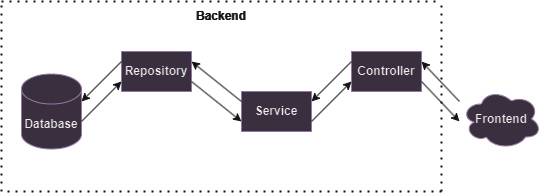
\includegraphics[width=14.0truecm]{images/BackendArchitecture.png}
\end{center}